%optimisation
\mysection{Le camion citerne}{Enigmath}{7 janvier 2026}
\begin{center}
    \includegraphics[width=0.4\textwidth]{\currfiledir/image.jpg}
\end{center}
\subsection*{Énoncé}
Un camion citerne d'une capacité maximale de \(1000\) litres doit transporter de l’essence de la ville \(A\) à la ville \(B\), distantes de \(1000\) km. La particularité de ce camion est qu'il consomme pour rouler l'essence qu'il transporte.
\begin{itemize}
\item Le camion consomme \(1\) litre par km parcouru.
\item Il peut déposer des bidons d’essence (en quantité et capacité illimitées) sur la route et les récupérer plus tard.
\end{itemize}

\medskip
\textbf{Questions} :
\begin{enumerate}
    \item\indicators{2.3}{0} Le dépôt initial en \(A\) contient \(3000\) litres. Quelle est la quantité maximale d’essence que le camion peut amener en \(B\) ?
    
    \item\indicators{2.1}{0} Quel est le stock minimal requis en \(A\) pour permettre au chauffeur de rapporter \(1000\) litres d’essence en \(B\) ?
    
    \item\indicators{2.1}{0} Exprimez la quantité maximale d’essence que le camion peut amener en \(B\) en fonction du stock disponible en \(A\).
\end{enumerate}

\subsection*{Solution}
\begin{enumerate}
    \item On suppose que le camion part de l’origine (la ville $A$) et se déplace le long de l’axe des abscisses positives.
On choisit comme \emph{unité de carburant} la quantité maximale que le camion peut transporter ; ainsi, toutes les quantités de carburant sont exprimées en milliers de litres et cette unité est appelée une \emph{charge}.  

La figure suivante donne une représentation schématique d’un trajet typique.
Le chemin représente les déplacements successifs du camion. Bien entendu,
en réalité, ce trajet est entièrement contenu sur l’axe des abscisses ; il a été
déformé verticalement uniquement afin d’en faciliter la visualisation.  
La longueur de ce chemin est alors précisément égale à la quantité totale de
carburant consommée. Sur la figure, le camion atteint un point situé à une distance $d$ de l’origine.

\begin{center}
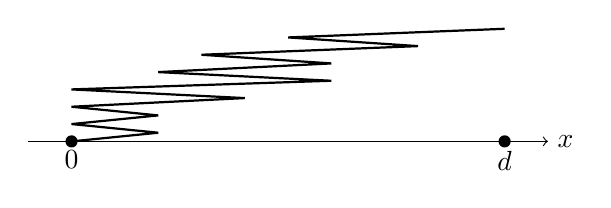
\begin{tikzpicture}[scale=1.1]

% Axe des x
\draw[->] (-0.5,0) -- (5.5,0) node[right] {$x$};

% Origine
\fill (0,0) circle (2pt);
\node[below] at (0,0) {$0$};
\fill (5,0) circle (2pt);
\node[below] at (5,0) {$d$};

% Trajet du camion
\def\xo{0.1}
\draw[thick] 
(0, 0) -- 
(1, 1*\xo) -- 
(0, 2*\xo) -- 
(1, 3*\xo) -- 
(0, 4*\xo) -- 
(2, 5*\xo) -- 
(0, 6*\xo) -- 
(3, 7*\xo) -- 
(1, 8*\xo) -- 
(3, 9*\xo) -- 
(1.5, 10*\xo) -- 
(4, 11*\xo) -- 
(2.5, 12*\xo) -- 
(5, 13*\xo);
\end{tikzpicture}
\end{center}
    
On cherche à établir une expression explicite de la fonction \(q(f)\), qui
désigne la quantité maximale d'essence que le camion peut amener en~$B$ (le point d’abscisse égale à $1$) en disposant de
\(f \ge 1\) charges de carburant en $A$ (pour cette question, on a donc $f=3$). Pour ce faire, on définit la distance maximale $d(f)$ que le camion peut atteindre. On a toujours $q(f) \ge d(f) - 1$. En effet, si le camion dispose d'une stratégie pour aller en $d(f)$, 
alors on peut modifier la stratégie de sorte que toute consommation de carburant effectuée
au-delà du point $B$ (cette consommation est donc supérieur à $d(f)-1$) peut être remplacée par un dépôt de carburant en $B$. On a aussi $1+d(q(f)) \le d(f)$, car une fois la stratégie d’acheminement d’une quantité $q(f)$ de carburant
jusqu’en $B$ réalisée, ce carburant peut être employé de la même manière qu’un stock initial pour permettre au camion de parcourir une distance supplémentaire
de $d(q(f))$. Si $d(f) \le 2$, alors $d(q(f)) \le 1$ et $q(f) \le 1$.\footnote{
En effet, avec un stock initial strictement supérieur à $1$, le camion peut
atteindre une distance strictement supérieure à $1$. Plus précisément, si l’on
dispose d’un stock initial égal à $1+\varepsilon$, on peut procéder de la manière
suivante. Lors d’un premier aller-retour effectué avec le camion plein, on dépose une
quantité
\(
1-\frac{2\varepsilon}{3}
\)
de carburant à une distance
\(
\frac{\varepsilon}{3}
\)
de l’origine.
Lors du second trajet, le camion part avec la charge restante $\varepsilon$. Il
consomme $\frac{\varepsilon}{3}$ pour atteindre le dépôt, et arrive donc avec
\(
\frac{2\varepsilon}{3}
\)
de carburant. En récupérant le carburant déposé, il dispose alors exactement
d’une charge complète.
Le camion peut ainsi parcourir une distance supplémentaire de $1$, ce qui lui
permet d’atteindre
\(
1+\frac{\varepsilon}{3}.
\)
} On dispose donc d'une stratégie pour aller en $1+q(f)$, et donc $1+q(f) \le d(f),$ i.e., on a l'égalité $q(f) = d(f) - 1.$ 
On se concentre donc, pour l’instant, sur l’étude de la fonction $d(f)$, et on va démontrer la formule (pour $f$ entier)
\[
d(f) = 1 + \frac{1}{3} + \frac{1}{5}  + \cdots + \frac{1}{2f-1},
\]
En particulier, on a $d(3) = 1 + \frac{1}{3} + \frac{1}{5} \le 2$, donc $q(3)=d(3)-1$ et la réponse à la question est environ 533.3 litres.

L’idée centrale de la démonstration consiste à utiliser une formule due à
Banach concernant la longueur d’un chemin dans un espace unidimensionnel. Pour exploiter la formule de Banach, on définit, pour chaque point
\(x \geq 0\), la \emph{valence} \(n(x)\) comme le nombre total de fois où le
camion passe par le point \(x\) au cours de son trajet (quel que soit le sens de
parcours).

La figure suivante représente le graphe de la fonction \(n(x)\)
associée au trajet schématisé précédemment.

\begin{center}
\begin{tikzpicture}[scale=1.1]
\def\yo{0.5}
% Axes
\draw[->] (-0.5,0) -- (5.5,0) node[right] {$x$};
\draw[->] (0,0.0) -- (0,8*\yo) node[above] {$n(x)$};

% Marches de la fonction n(x)
\fill (0,4*\yo) circle (2pt);
\draw[thick] (0,7*\yo) -- (1,7*\yo);
\fill (1,6*\yo) circle (2pt);
\draw[thick] (1,5*\yo) -- (1.5,5*\yo);
\fill (1.5,6*\yo) circle (2pt);
\draw[thick] (1.5,7*\yo) -- (2,7*\yo);
\fill (2,6*\yo) circle (2pt);
\draw[thick] (2,5*\yo) -- (2.5,5*\yo);
\fill (2.5,6*\yo) circle (2pt);
\draw[thick] (2.5,7*\yo) -- (3,7*\yo);
\fill (3,5*\yo) circle (2pt);
\draw[thick] (3,3*\yo) -- (4,3*\yo);
\fill (4,2*\yo) circle (2pt);
\draw[thick] (4,1*\yo) -- (5,1*\yo);

\node[below] at (0,0) {$0$};
\draw[thick] (5,-.05) -- (5,.05);
\node[below] at (5,0) {$d$};

% Valeurs de n(x)
\node[left] at (0,1*\yo) {$1$};
\node[left] at (0,2*\yo) {$2$};
\node[left] at (0,3*\yo) {$3$};
\node[left] at (0,4*\yo) {$4$};
\node[left] at (0,5*\yo) {$5$};
\node[left] at (0,6*\yo) {$6$};
\node[left] at (0,7*\yo) {$7$};

\end{tikzpicture}
\end{center}

La formule de Banach affirme
que la longueur du chemin pour atteindre $d$ (i.e., la quantité totale de carburant consommée pour atteindre $d$) est donnée par
\[
\text{longueur du chemin pour atteindre }d
= \int_0^{d} n(x)\,dx.
\]

Pour tout trajet du camion permettant d'atteindre un point situé à une distance $d$ de l'origine, on définit $x_t$ comme le point de $[0,d]$ tel que la longueur totale du
trajet à droite de $x_t$ soit
exactement égale à $t$.
Par exemple,  $x_f = 0$ et $x_0=d$. La fonction $t\mapsto x_t$ est strictement décroissante, et
il y a exactement $a$ unités de longueur entre $x_{t+a}$ et
$x_t$, i.e., $\int_{x_{t+a}}^{x_t}n(x)dx = a$.

\begin{lemma}[Gale]
Pour $k\in \mathbb{N}$, $k\le f$, si $x < x_k$, alors
\[
n(x) \ge 2k+1.
\]
\end{lemma}

\begin{proof}
Puisque $x$ se situe à gauche de $x_k$, le camion doit consommer plus de $k$
charges de carburant à droite de $x$.  
Comme le camion ne peut transporter qu’une charge à la fois, il doit donc traverser
le point $x$ au moins $k+1$ fois en venant de la gauche.  

Mais entre deux passages consécutifs depuis la gauche, il doit y avoir un
passage depuis la droite. Il y aura donc au moins $k$ passages depuis la droite.  

On obtient ainsi que le camion doit passer au moins $2k+1$ fois par le
point $x$.
\end{proof}


Nous combinons maintenant ce résultat avec la formule de Banach :
\[
1=\int_{x_{k+1}}^{x_k} n(x)\,dx
\ge (2k+1)(x_k - x_{k+1}),
\]
d’où l’inégalité
\[
x_k - x_{k+1} \le \frac{1}{2k+1}.
\]

En sommant cette inégalité pour $k=0$ à $f-1$, on obtient
\[
d = x_0 - x_f
= \sum_{k=0}^{f-1} (x_k - x_{k+1})
\le \sum_{k=0}^{f-1} \frac{1}{2k+1}
= 1 + \frac{1}{3} + \frac{1}{5} + \cdots + \frac{1}{2f-1},
\]
ce qui fournit une borne supérieure pour 
$d(f)$.
    
Il reste seulement à montrer que cette borne peut être atteinte, ce qui se fait
aisément par récurrence.
La formule est manifestement correcte pour $f=1$. Supposons-la maintenant vraie
pour un certain entier $f \ge 1$, et considérons le cas de $f+1$ charges. Le camion commence par transporter ces $f+1$ charges jusqu’au point situé à la
distance
\(
\frac{1}{2f+1}
\)
de l’origine. Cette opération nécessite $f+1$ trajets aller et $f$ trajets retour,
soit au total $2f+1$ parcours de longueur $\frac{1}{2f+1}$. La consommation totale
est donc exactement égale à une charge. Il reste alors $f$ charges de carburant déposées en ce point. D’après l’hypothèse
de récurrence, la distance maximale que le camion peut encore parcourir à partir
de ce point est
\[
1 + \frac{1}{3} + \frac{1}{5} + \cdots + \frac{1}{2f-1}.
\]

On en déduit que, avec $f+1$ charges, le camion peut atteindre la distance
\[
\frac{1}{2f+1}
+ 1 + \frac{1}{3} + \frac{1}{5} + \cdots + \frac{1}{2f-1}
= 1 + \frac{1}{3} + \frac{1}{5} + \cdots + \frac{1}{2(f+1)-1},
\]
ce qui établit la formule au rang $f+1$ et achève la démonstration.

\item On cherche le $f$ tel que $q(f)=1$. Comme $q(f)\ge d(f)-1$, on a $d(f) \le 2$ et donc, comme à la question précédente, $q(f)=d(f)-1.$
Pour $f$ non entier, on a
\[d(f) = 1 + \frac{1}{3} + \cdots + \frac{1}{2\lfloor f\rfloor-1} + \frac{f-\lfloor f\rfloor}{2\lfloor f\rfloor + 1}.\]
En effet, comme $n(x)\geq 2\lfloor f\rfloor + 1$ pour $x<x_{\lfloor f\rfloor}$, on a $$f-\lfloor f\rfloor = \int_{x_f}^{x_{\lfloor f\rfloor}}n(x)dx \geq (2\lfloor f\rfloor + 1)(x_{\lfloor f\rfloor}-x_f),$$
et donc
\[d = x_0 - x_f = x_{\lfloor f\rfloor}-x_f+\sum_{k=0}^{\lfloor f\rfloor-1}(x_k-x_{k+1})
\le \frac{f-\lfloor f\rfloor}{2\lfloor f\rfloor + 1}+\sum_{k=0}^{\lfloor f\rfloor-1} \frac{1}{2k+1}.\]
Pour montrer que cette borne est atteinte, on peut voir qu'il est possible d'amener $\lfloor f\rfloor$ unités en position $\frac{f-{\lfloor f\rfloor}}{2{\lfloor f\rfloor}+1}$, avec ${\lfloor f\rfloor}$
trajets aller et ${\lfloor f\rfloor}$ trajets retour.
Puis, lors d'un dernier trajet aller, on peut amener le surplus $f-{\lfloor f\rfloor}$.
On a donc au total $2{\lfloor f\rfloor}+1$ parcours de longueur $\frac{f-{\lfloor f\rfloor}}{2{\lfloor f\rfloor}+1}$.
La consommation totale est donc exactement égale à $f-{\lfloor f\rfloor}$, et il reste $\lfloor f\rfloor$ charges en position $\frac{f-{\lfloor f\rfloor}}{2{\lfloor f\rfloor}+1}$. On peut enfin appliquer le cas d'un stock initial entier pour conclure.

Comme $1/3+1/5+1/7+1/9+1/11+1/13<1$ et $1/3+1/5+1/7+1/9+1/11+1/13+1/15>1$, on cherche $f$ tel que $\lfloor f\rfloor=7$ et $f-\lfloor f\rfloor = 15(1-(1/3+1/5+1/7+1/9+1/11+1/13))$, i.e., $f=\frac{23042}{3003}$. Cela correspond à environ $7673$ litres.

\item La fonction $d$ est continue, strictement croissante. Elle admet donc une fonction réciproque. On va démontrer la formule 
\[q(f) = d^{-1}(\max(0,d(f)-1)).\]
Au passage, une procédure pour calculer $d^{-1}$ est la suivante :
pour une valeur donnée de $d$, on commence par déterminer l’unique entier
$n \in \mathbb{N}$ tel que
\[
\sum_{k=0}^{n-1} \frac{1}{2k+1}
\;\le\;
d
\;<\;
\sum_{k=0}^{n} \frac{1}{2k+1}.
\]
Alors la valeur correspondante de $f$ est donnée par
\[
f
=
n
+
(2n+1)\!\left(
d
-
\sum_{k=0}^{n-1} \frac{1}{2k+1}
\right).
\]

Si $f\le 1$, $d(f)=f$ et $q(f)=d^{-1}(0)=0$. Si $f > 1,$ $d(f) > 1$ et il suffit de montrer que
\[1+d(q(f)) = d(f).\]
On peut supposer, sans perte d'optimalité, qu'il existe une station en $B$
($x=1$). En effet, pour tout trajet atteignant la distance $d(f)$, toute
consommation de carburant effectuée au-delà de~$B$ peut être remplacée par un
dépôt de carburant en $B$. Une fois ce dépôt constitué, les trajets situés au-delà
de $B$ peuvent être reproduits dans le même ordre qu'auparavant en utilisant le
carburant stocké en $B$, sans modifier la distance maximale atteinte.
Si l’on note $q$ la quantité de carburant déposée en $B$, on a alors
\(
d(f)=1+d(q)\le 1+d(q(f)).
\)
Comme on sait déjà que
\(
1+d(q(f))\le d(f),
\)
on en déduit l’égalité.
\end{enumerate}

\subsection*{Notes et références}
Le \emph{problème du jeep}, aussi appelé \emph{problème de la traversée du désert}
ou \emph{problème de l’exploration}, est une énigme classique d’optimisation
logistique consistant à maximiser la distance parcourue par un véhicule disposant
d’une capacité limitée en carburant, mais autorisé à créer des dépôts intermédiaires.
Ce problème apparaît dès le IX\textsuperscript{e} siècle dans le recueil
\emph{Propositiones ad Acuendos Juvenes}, attribué à Alcuin, sous la forme d’un
problème de chameau transportant des vivres. Il est également étudié par Luca
Pacioli dans \emph{De viribus quantitatis} vers 1500. Une formulation moderne et
mathématiquement rigoureuse est donnée par N.~J.~Fine en 1947 \cite{fine1947jeep}, qui introduit le
modèle du jeep traversant le désert et en donne une solution optimale. Peu après,
C.~G.~Phipps généralise le problème au cas d’une caravane de plusieurs jeeps \cite{phipps1947jeep},
ouvrant la voie à de nombreuses variantes. Des contributions notables sont également dues à L.~Alaoglu, I.~Niven
et D.~Gale, ce dernier proposant une solution \cite{gale1970jeep} élégante fondée sur une formule de
Banach pour la longueur des trajectoires. Pour la présente solution, nous nous appuyons principalement sur les travaux de
D.~Gale.

\bibliography{\currfiledir/sources.bib}
\newpage